\documentclass[10pt]{article}
\usepackage[margin=1.2in]{geometry}
\usepackage[utf8]{inputenc}
\usepackage[english]{babel}
\usepackage[T1]{fontenc}
\usepackage{fourier}
\usepackage{amsthm}
\usepackage{amssymb}
\usepackage{amsmath}
\usepackage{amsfonts}
\usepackage{latexsym}
\usepackage{graphicx}
\usepackage{float}
\usepackage{etoolbox}
\usepackage{hyperref}
\usepackage{tikz}
\usepackage{lipsum}
\usepackage{svg}
\usepackage{algorithm}
\usepackage{algpseudocode}
\usepackage{mathtools}
\usepackage{nccmath}
\usepackage[most]{tcolorbox}
\newtcolorbox[auto counter]{problem}[1][]{%
    enhanced,
    breakable,
    colback=white,
    colbacktitle=white,
    coltitle=black,
    fonttitle=\bfseries,
    boxrule=.6pt,
    titlerule=.2pt,
    toptitle=3pt,
    bottomtitle=3pt,
    title=GitHub repository of this project}

\newcommand{\R}{\mathbb{R}}
\newcommand{\N}{\mathbb{N}}
\newcommand{\Z}{\mathbb{Z}}
\newcommand{\Q}{\mathbb{Q}}
\newcommand{\C}{\mathbb{C}}


\title{Assignment 1: The softmax function}
\author{Luca Lombardo}
\date{\today}

\begin{document}
\maketitle

% \tableofcontents

\setlength{\parindent}{0em}
% \setlength{\parskip}{1em}

% \section{Introduction}
% The softmax function is a mathematical function that takes a vector of real numbers as input and transforms it into a probability distribution. The mathematical definition of the softmax function is given by:

% \begin{equation*}
%     \sigma: \R^K \to \Big\{ z \in \R^K \,|\, z_i \geq 0, \sum_{i=1}^K z_i = 1 \Big\}
% \end{equation*}
% \begin{equation}
%     \sigma(\mathbf{z}_j) = \frac{e^{z_j}}{\sum_{i=1}^K e^{z_i}}
% \end{equation}

\section{Implementations}
In the following sections, given a scalar implementation (to witch we will refer as \texttt{softmax\_plain}), we will show how to auto-vectorize it and then how to manually vectorize the code using AVX intrinsics and FMA. Then we will compare the results of the three implementations.

\subsection{Auto-Vectorized implementation}
In implementing\footnote{This version is implemented in the file \texttt{softmax\_auto.cpp}.} the autovectorized version of the softmax function, I made several key modifications compared to the plain implementation. First, I added \texttt{\#pragma omp simd} directives to explicitly instruct the compiler to vectorize the three main computational loops, allowing parallel processing of multiple array elements with SIMD instructions. For the first two loops, I included appropriate reduction clauses (i.e., \texttt{reduction(max : max\_val)} and \texttt{reduction(+ : sum)}) to ensure correct calculation of the maximum value and sum while maintaining vectorization. I replaced \texttt{std::exp()} with the single-precision \texttt{expf()} function, which is specifically optimized for floating-point operations, offers better performance with SIMD instructions, and avoids unnecessary double-precision calculations that would be performed by \texttt{std::exp()} before converting back to float. Rather than using repeated divisions in the normalization step, I precomputed the inverse of the sum (\texttt{inv\_sum = 1.0f / sum}) and used multiplication operations, which are generally more efficient in vectorized code. Instead of using \texttt{std::max()}, I implemented an explicit comparison with an \texttt{if}-statement that might be more amenable to autovectorization for the compiler. \\

It is worth noting that replacing \texttt{\#pragma omp simd} with \texttt{\#pragma omp parallel for simd} results in significantly degraded performance for small values of K (becoming even slower than the plain implementation). This counterintuitive behavior occurs because thread creation and management introduce considerable overhead that outweighs any computational benefits when processing small arrays. The cost of spawning threads, synchronizing their execution, and handling potential load imbalances becomes expensive relative to the limited work being performed. On the other hand, fot large values of K, the parallelized version scales well: the computation workload here is sufficiently large to justify the overhead of thread management, and the performance gains from parallel execution become evident.

\subsection{Manually Vectorized implementation}
In designing the softmax implementation, I developed two distinct versions to address different input size scenarios. For large input arrays, the primary variant employs cache blocking with a block size derived from the L1 cache capacity (4096 bytes) to ensure that each data block remains in cache during processing. This decision minimizes memory latency through effective prefetching and loop unrolling, while OpenMP parallelization distributes the computational load across threads. In contrast, the "small" version avoids the overhead associated with thread management and cache blocking, which is unnecessary for data sizes that already reside in cache. This dual-approach allows the implementation to achieve optimal performance: the large variant excels with high data volumes where memory access becomes the bottleneck, and the small variant delivers better throughput for cache-resident datasets. \\

For the primary function, several specific optimization choices were made to maximize efficiency. Data is processed in chunks of 32 elements per iteration to match the width of AVX registers, and for indices not multiple of 8, scalar processing is used rather than vector masking; the infrequent residual iterations render the simpler scalar approach both effective and low-overhead. The use of the \texttt{\_mm256\_fnmadd\_ps} intrinsic in the exponential computation phase was carefully integrated to combine the subtraction of the maximum value with the preparation of the exponent input in one step, thereby reducing the overall instruction count and streamlining the computation pipeline.

\section{Results}
In the following section we will compare the three implementations of the softmax function under different conditions. There 2 main parameters that we will vary: the machine architecture (one supporting AVX512 and one not supporting it) and the parallelization in the implementation of \texttt{softmax\_auto}. The two differnt machine architectures are:
\begin{itemize}
  \item \textbf{Machine 1}: Intel(R) Xeon(R) Gold 5318Y, 96 threads, 1TB RAM.
  \item \textbf{Machine 2}: AMD Ryzen 5 PRO 5650G, 12 threads, 32GB RAM.
\end{itemize}
Both running Ubuntu 22.04 LTS. \\

The importance of the AVX512 instruction set is crucial in comparing the performance of \texttt{softmax\_auto} and \texttt{softmax\_avx}. The \texttt{softmax\_auto} implementation relies on the compiler's ability to auto-vectorize the code, which will use AVX512 instructions if available. Thus comparing the performance of \texttt{softmax\_auto} with AVX512 support against the \texttt{softmax\_avx} implementation, which is manually optimized for AVX2, will be clearly unbalanced. We expect the \texttt{softmax\_auto} implementation to outperform the \texttt{softmax\_avx} implementation on the machine with AVX512 support, while the opposite is expected on the machine without AVX512 support.

\paragraph{How do we measure the performance?}
Performance is measured using a rigorous benchmark: after 3 warmup iterations, 11 samples (each averaging 20 iterations) are taken and the median is reported. Input sizes vary from 1 to 1,048,576 elements (both powers of 2 and non-power-of-2) to test alignment. A custom C++17 aligned allocator (32-byte alignment) ensures fair SIMD comparisons. Correctness is verified by checking that each implementation produces equivalent probability distributions (non-negative values summing to 1), and speedups are reported relative to the plain implementation.

\subsection{Without AVX512 support on host}
Let's start with the results of the machine without AVX512 support. We first begin by comparing the results without the \texttt{parallel} directive in the \texttt{softmax\_auto} implementation. The results are shown in the following plot:

\begin{figure}[H]
  \centering
  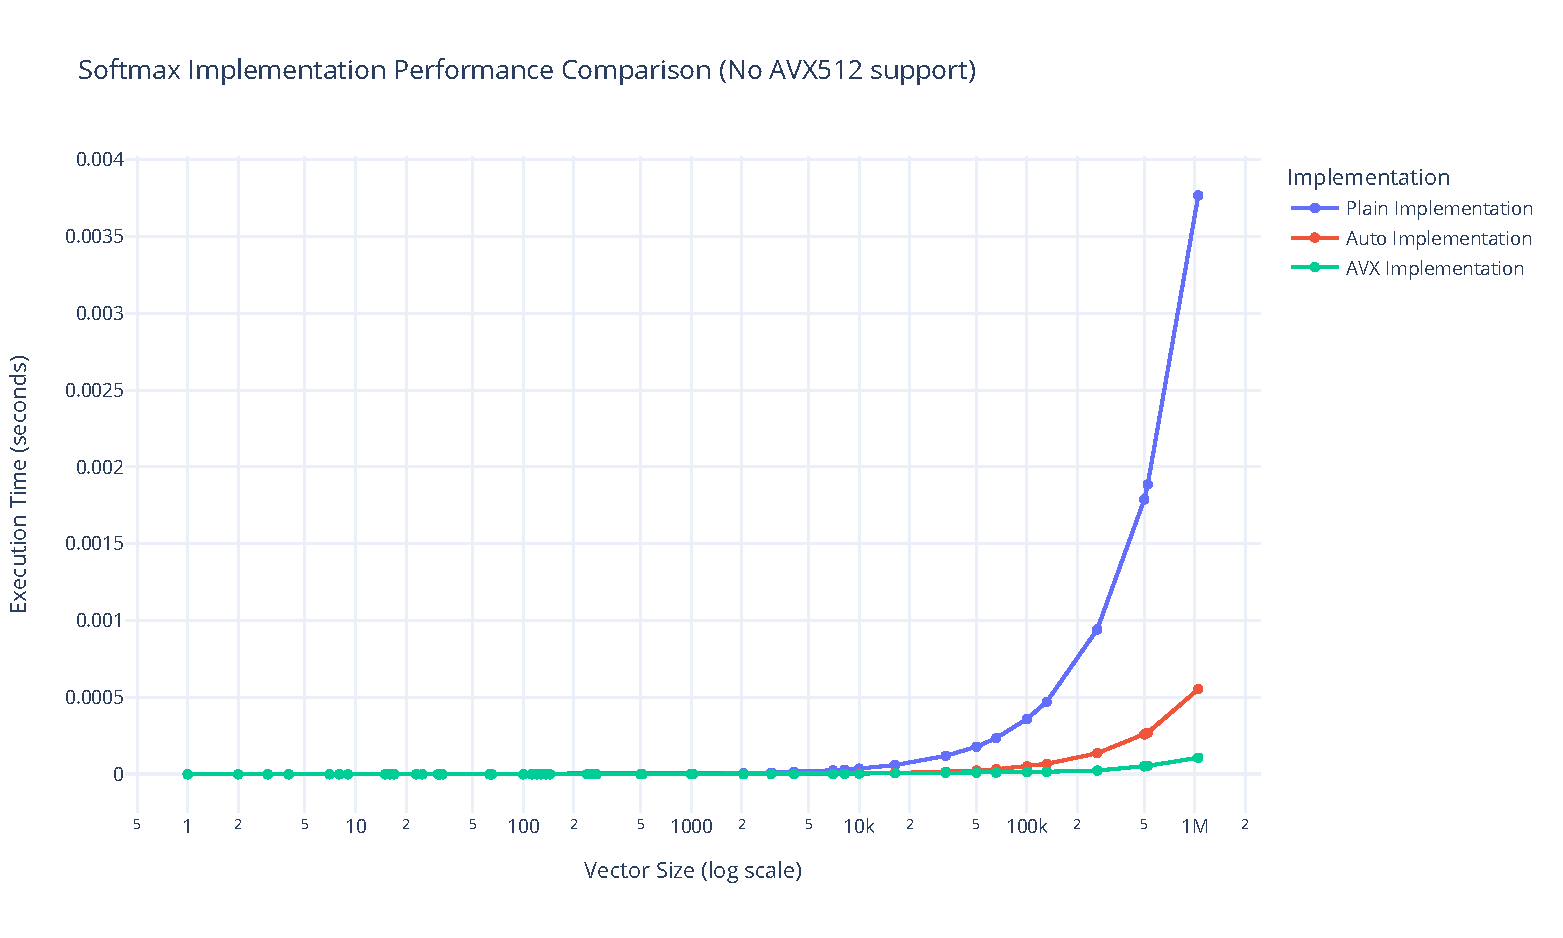
\includegraphics[width=0.8\textwidth]{../images/softmax_noparallel.pdf}
  \caption{Performance comparison of the three implementations of the softmax function without AVX512 support and without parallelization for \texttt{softmax\_auto}.}
  \label{fig:softmax_auto_no_parallel}
\end{figure}

We can clearly see that the \texttt{softmax\_avx} implementation outperforms the \texttt{softmax\_auto} implementation, which in turn outperforms the plain implementation. Let's see what happens when we add the \texttt{parallel} directive to the \texttt{softmax\_auto} implementation. The results are shown in the following plot:
\begin{figure}[H]
  \centering
  \includegraphics[width=0.8\textwidth]{../images/softmax_parallel.pdf}
  \caption{Performance comparison of the three implementations of the softmax function without AVX512 support and with parallelization for \texttt{softmax\_auto}.}
  \label{fig:softmax_auto_parallel}
\end{figure}



\end{document}
